\chapter{Results}
\label{chap:results}

\section{Interface}
As mentioned in the previous chapter, SketchMeshVR does not make use of any menus and instead solely relies on different combinations of button presses to differentiate between the multiple available modelling actions. This does require more effort from the user in order to keep track of the selected editing modes, but at the same time keeps the interface cleaner. In order to guide the user when drawing strokes, SketchMeshVR provides visual feedback on the positions that will be used to create a stroke. In case of the drawing and curve deformation modes this means that the user sees the position controller and in case of all other modes the user will see the position controller plus a ray shooting from it (the ray ends at any intersections it has with the scene). Figures~\ref{fig:interface}(a) and (b) show what this looks like.

\begin{figure}[!h]
    \centering
    \setlength{\tabcolsep}{0.0130\linewidth}
    \begin{tabular}{@{}cc@{}}
    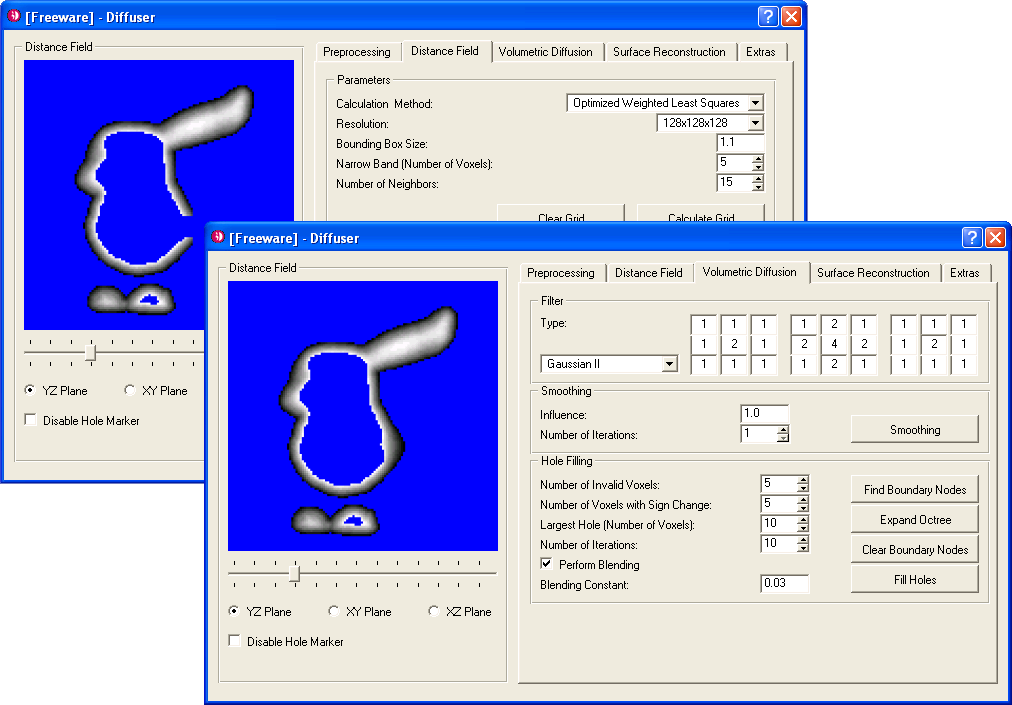
\includegraphics[width=0.3\linewidth]{figures/voldiff_ui}&
  	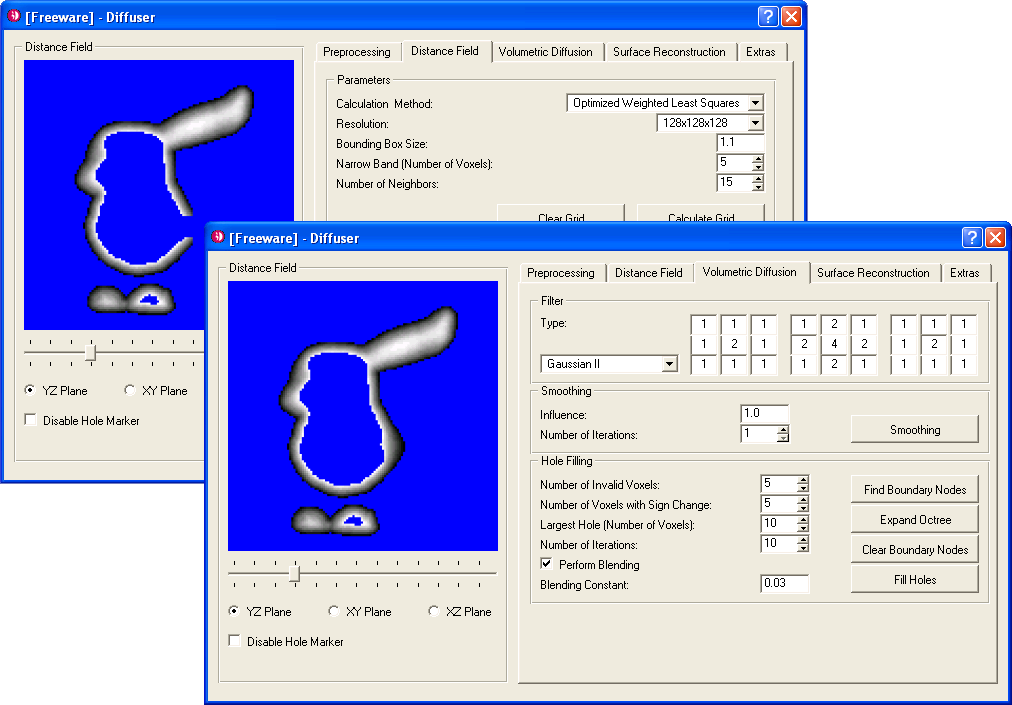
\includegraphics[width=0.3\linewidth]{figures/voldiff_ui}\\
    (a)&(b)\\
    \end{tabular}
    \caption[SketchMeshVR interface]{SketchMeshVR interface.
    	  \textup{(a)} Controller reference point that is displayed in drawing and deformation mode.
			  \textup{(b)} Controller and ray reference that are displayed in all other editing modes. 
      \label{fig:interface}}
\end{figure}
 
\section{User review}

\textcolor{red}{TODO:}
\begin{itemize}
\item mention test users' prior experience with 3D modelling and VR
\item explain test setup: asking users to recreate an example model both in VR \& non-VR version of program
\item summarize any comments they have on the test/experience
\item what did they think of ease of learning/modelling?
\item Is there a difference in efficiency between modelling in VR or non-VR?
\item show side-by-side comparisons of example model and user recreations
\end{itemize}


\begin{figure}[!h]
    \centering
    \setlength{\tabcolsep}{0.0130\linewidth}
    \begin{tabular}{@{}ccc@{}}
    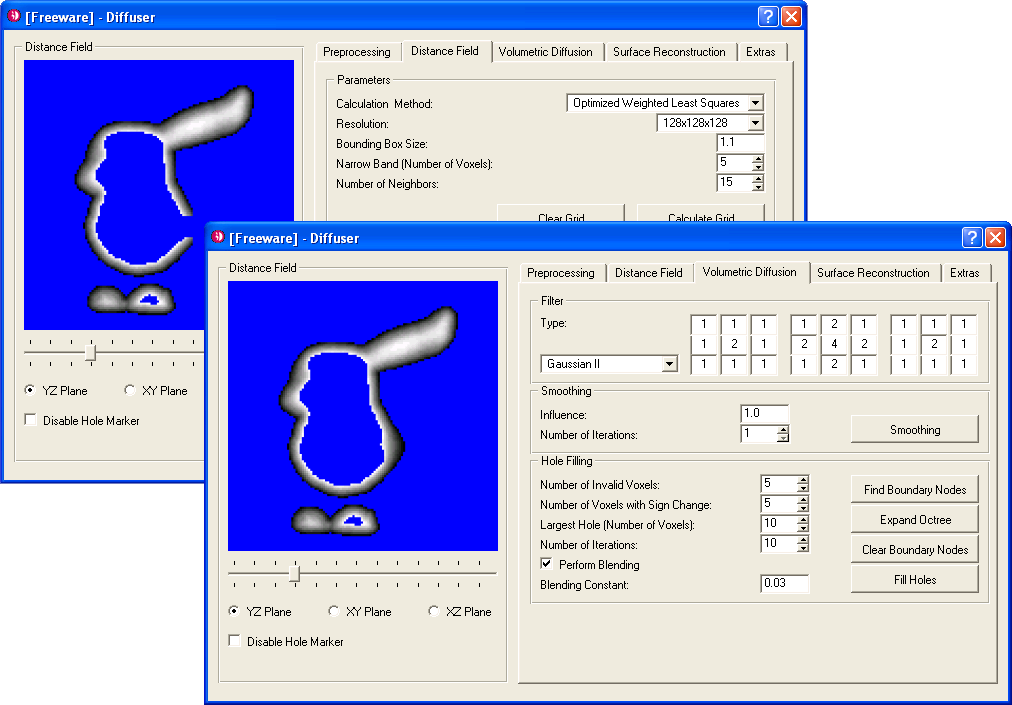
\includegraphics[width=0.3\linewidth]{figures/voldiff_ui}&
  	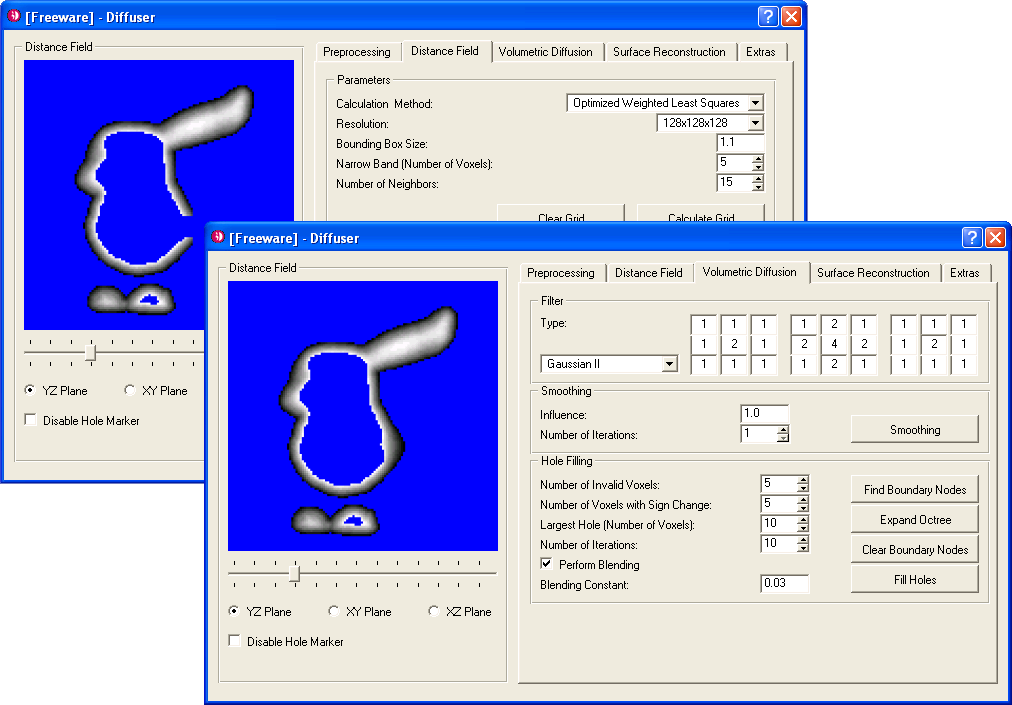
\includegraphics[width=0.3\linewidth]{figures/voldiff_ui}&
  	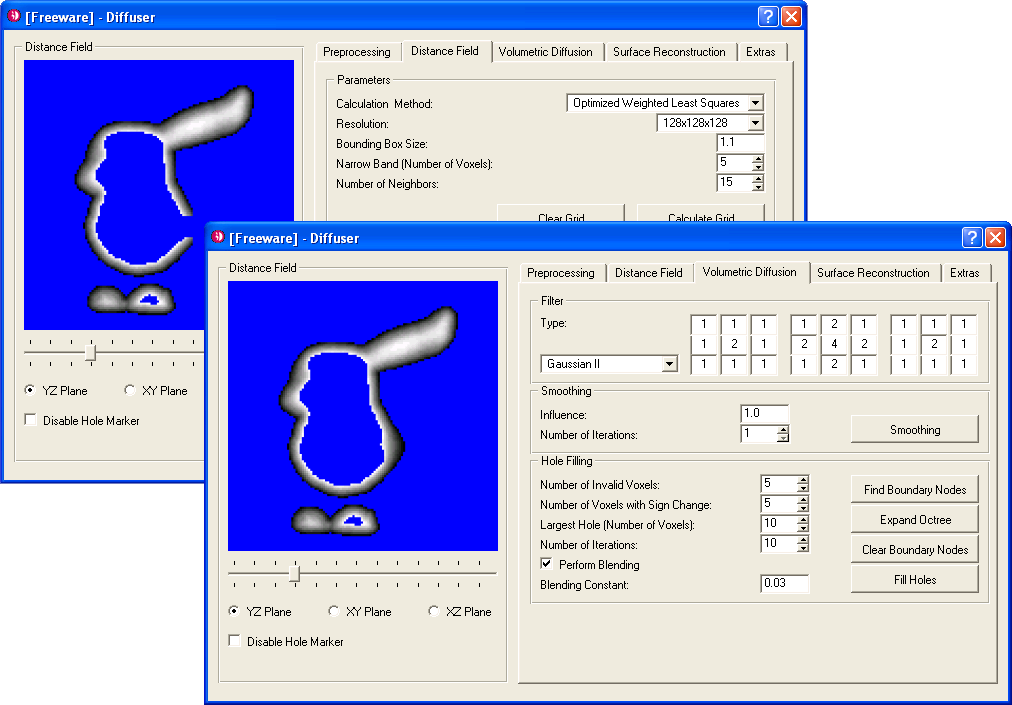
\includegraphics[width=0.3\linewidth]{figures/voldiff_ui}\\

    (a)&(b)&(c)\\
    \end{tabular}
    \caption[SketchMeshVR teddy model]{SketchMeshVR recreating models.
    	  \textup{(a)} Example simplified mesh of a teddy bear.
	  \textup{(b)} Resulting recreated model made in VR  (took X seconds to complete).
	  \textup{(c)} Resulting recreated model made in non-VR (took Y seconds to complete).
      \label{fig:recreate_teddy}}
\end{figure}
\todo{Fill in taken seconds in caption}


\begin{figure}[!h]
    \centering
    \setlength{\tabcolsep}{0.0130\linewidth}
    \begin{tabular}{@{}ccc@{}}
    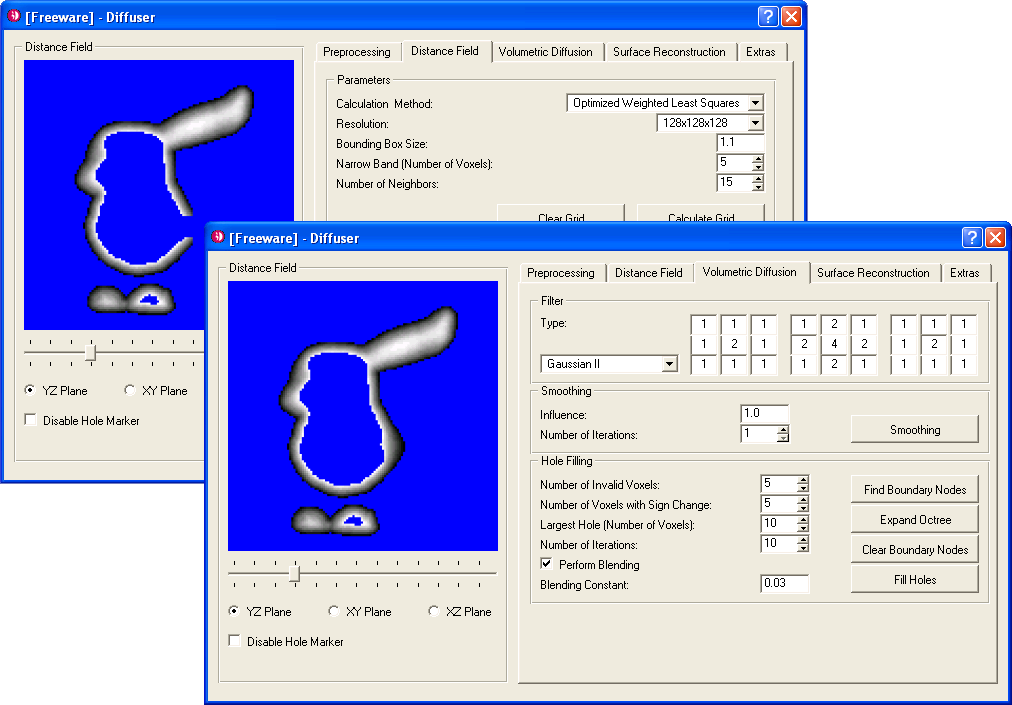
\includegraphics[width=0.3\linewidth]{figures/voldiff_ui}&
  	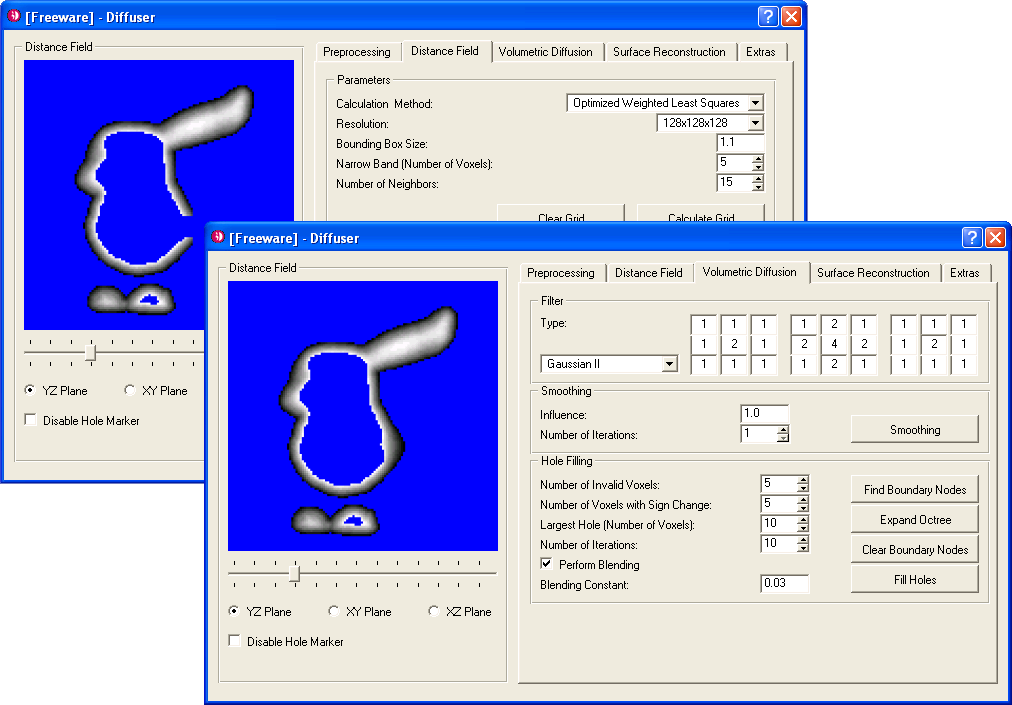
\includegraphics[width=0.3\linewidth]{figures/voldiff_ui}&
  	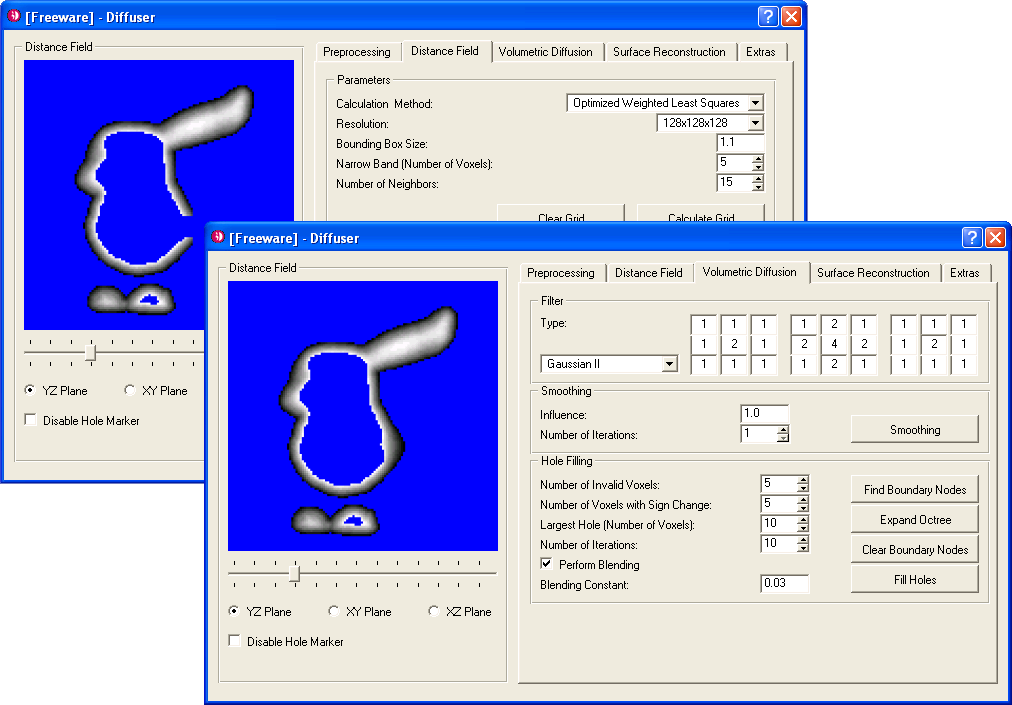
\includegraphics[width=0.3\linewidth]{figures/voldiff_ui}\\

    (a)&(b)&(c)\\
    \end{tabular}
    \caption[SketchMeshVR dolphin model]{SketchMeshVR recreating models.
    	  \textup{(a)} Example simplified mesh of a dolphin.
	  \textup{(b)} Resulting recreated model made in VR (took X seconds to complete).
	  \textup{(c)} Resulting recreated model made in non-VR (took Y seconds to complete).
      \label{fig:recreate_dolphin}}
\end{figure}
\todo{Fill in taken seconds in caption}